\documentclass[12pt]{paper}

\usepackage{Schwieg}
\usepackage[margin=1in]{geometry}
\usepackage{tikz}
\title{Price Theory I: Problem Set 1.2}
\author{Samuel Barker\and Timothy Schwieg\and Rafeh Qureshi\and Daniel Noriega\and Ana Vasilj}
\begin{document}
\maketitle

Given: there are two regions: north and south; the exterior temperature in the north ($T_N$) is always less than the exterior temperature in the south ($T_S$); people have preferences on one good $X$ and on the interior temperature of their house ($H$); people can raise $H$ by $K$ by spending $K*C(I)$ where $I$ is the amount of insulation and $C'(I)<0$; and finally that wages in a region depends negatively on the amount of people in that region.

Assumed: utility functions are of the same form for all individuals and are strictly quasi-concave; individuals are free to move between regions; and the ideal temperature is higher than the current external temperature in both north and south (i.e. everyone prefers higher temperatures for their houses relative to the exterior temperature).

\section{Part A}
Q: Assuming insulation in the north and south are fixed at the same level, how will wages, consumption of $X$, and $H$ differ?
\\

\textbf{Claim: $u(X_N,H_N)=u(X_S,H_S)$ in equilibrium.}

This follows from the fact that if $u_N>u_S$ then people would move north. Informally, this would result in $w_N$ falling and $w_S$ rising until $u_N=u_S$.
\\

\textbf{Claim: $X_N=X_S$ and $H_N=H_S$ in equilibrium.}

This claim follows from two facts: the utility functions are the same, and they face the same prices (i.e. $P_x$  and $ C(I)$. Because they face the same prices, the slope of the budget line is the same and the $X$ and $H$ for which they are tangent would have to be the same. We know that in equilibrium the slope of the budget line is the same as the slope of the line tangent to the utility curve and, by strict quasi-concavity, this spot on the utility curve is unique. Thus there is a unique $X^*$ and $H^*$ such that $u^{'}_i(X^*,H^*)=\frac{C(I)}{P_X},~i\in  \{N,S\}$ (where the right hand side is the slope of the budget line).
\\

\textbf{Claim: $K_N>K_S$, $w_N>w_S$, and there are more people in the south than in the north.}

The first fact comes immediately from $H^*=H_N=H_S.$ Notice that $H_N=T_N+K_N=T_S+K_S=H_S$, and we know that $T_S>T_N \implies K_N>K_S$.

The second fact follows from the first. In equilibrium $w_i=P_XX_i+C(I)K_i^*. $ It follows that:
\begin{align*}
K_N&>K_S\\
K_NC(I)&>K_SC(I)\\
P_XX+K_NC(I)&>P_XX+K_SC(I)
\end{align*}
These are just the budget constraints for the north and south respectively. We know that in equilibrium, wage will be equal to total expenditure, and thus:
\begin{align*}
w_N=P_XX+K_NC(I)&>P_XX+K_SC(I)=w_S\\
\implies w_N&>w_S.
\end{align*}

Since it is given that wages are negatively related to the population of a region. Therefore, we get our third result: there are more people in the south than the north because $w_N>w_S$. (See Figure 1)


\section{Part B}
Q: What will happen to wages and house temperatures in both regions if there is an equal increase in insulation in both places?
\\

To model this, imagine that insulation has been added to houses and wages have not adjusted yet. Denote the state before the insulation increase as state $0$, and after as state $1$.

If wages have not adjusted yet, then: 
\begin{align*}
w_{N_1}-w_{N_0}=0&=w_{S_1}-w_{S_0}\\
w_{N_1}-w_{N_0}=&~w_{S_1}-w_{S_0}
\end{align*}
Because wages will equal expenditure, we also have:
\begin{align*}
P_XX_1+C(I_1)K_{N_1}-P_XX_0-C(I_0)K_{N_0}&=P_XX_1+C(I_1)K_{S_1}-P_XX_0-C(I_0)K_{S_0}
\end{align*}
Realize that because north and south face a budget constraint with the same slope again, there once again exists a unique $X^*_1$ such that the slope for $u$ at that point is equal to the budget line in both regions. This implies that $X_{N_1}=X_{S_1}$, which is why a general $X_1$ has been used. This also means that we can cancel out $P_XX_0$ and $P_XX_1$ from each side. We then get:
\begin{align*}
C(I_1)K_{N_1}-C(I_0)K_{N_0}&=C(I_1)K_{S_1}-C(I_0)K_{S_0}\\
C(I_1)(K_{N_1}-K_{S_1})&=C(I_0)(K_{N_0}-K_{S_0})
\end{align*}
Because $C'(I)<0$, and $I_1>I_0$, we have that $C(I_1)<C(I_0)$. This implies that:
\begin{align*}
K_{N_1}-K_{S_1}&>K_{N_0}-K_{S_0}
\end{align*}
The reason we know that the inequality goes this direction, is because we have that $K_{N_0}>K_{S_0}$. The important result from this is the difference between household temperature in the north and south is no longer equal after the insulation increase--this is the income effect. However, we established that consumption of $X$ in north and south is equal. Thus, if $H_{N_1}>H_{S_1}$, we would have that $u(X,H_{N_1})>u(X,H_{S_1}).$


A person can get more utility in the north right after the increase in insulation. Utility maximizing people would then move to the north, causing the wage in the north to fall, and the wage in the south to rise until the utilities equalize. When the utilities are equal, the binary relations from Part A still hold. Namely: $X$ is the same for north and south; $H$ will be the same for north and south; wages in the south are lower than in the north;  $K_N>K_S$; and the number of people in the south is greater than in the north. However, with an increase in $I$, the wage gap (and therefore population gap) between north and south will be smaller; both will spend more on $K$ and less on $X$ (substitution effect, and obvious from the budget line slope change (See Figure 2)). Both the north and south utilities would have increased.

\section{Part C}
Q: Assuming that the quantity of insulation can be adjusted at a fixed price $P_I$, how will the amount of insulation used, interior temperatures, energy costs, and consumption of $X$ differ now?
\\

From part B: the north's marginal benefit from $C(I)$ is higher, as for a given $I$ increase in both regions the north's utility would increase more than the south's. Thus, we can infer that, in equilibrium, people in the north will be using more insulation than people in the south, as the north will relatively benefit more from insulation.
Consequently, the slope of the people in the north's budget line $(P_x/C(I))$ will be flatter (see Figure 3), and therefore, $H_N>H_S$ and $X_N<X_S$. Similarly, $K_N$ will increase relative to $K_S$.
  
In part B, we concluded that the north benefits more from a given increase in insulation, relative to the south, because they were spending more in $K$ than the south. Thus, we can conclude that, for any given $P_I$, the north would be buying more insulation than the south.

We also can show that, if we consider a budget line in a two dimension graph, with $X$ on the $y$ axis and $K$ on the $x$ axis, more insulation would make this budget line flatter (wage fixed). To see that, take amounts of insulation $I_1>I_0$ and consider $w^0=w-I^0P_I$ and $w^1=w^0-dIP_I$, where $dI$ is a positive variation in I. Then, the intercept of the budget line with the $x$ axis in $I^0$ is just $\frac{w^0}{C(I^0)}$ and in $I^1$, it intercepts at $\frac{w^1}{C(I^1)}$. the we have:
\begin{equation}
\begin{split}
\frac{w^1}{C(I^1)}&=\frac{w^0}{C(I^0)+C'(I^0)dI}-\frac{P_IdI}{C(I^0)+C'(I^0)dI}\\
&\ge \frac{w^0}{C(I^0)+C'(I^0)dI}>\frac{w^0}{C(I^0)}
\end{split}
\end{equation}
\noindent where the inequalities come from $C'(.)<0$ and also $C(I^0)+C'(I^0)dI>0$. The latter is also a reasonable assumption, since it comes from decreasing marginal returns from buying insulation (i.e., $C'(.)\to 0$ as its argument increases).

Knowing that and that the utility functions are the same for people in the north and in the south (except that people in the north have a flatter budget line), we can conclude that the spot where the slope of the budget line of the north is equal an indifference curve is lower (i.e., has more $K$ and less $X$ than where the budget line for the south has the same slope as the indifference curve). Also, because any adjustments made in wages when people move just result in parallel shifts in the budget lines, the conclusions about the slopes remain the same, even after we allow wages to adjust in equilibrium. Therefore, we can also conclude that people in the north will consume more $I$ and more $K$, which results in lower $C(I)$, relative to people in the south, but people in the south would consume more $X$ relative to people in the north.


\begin{figure}
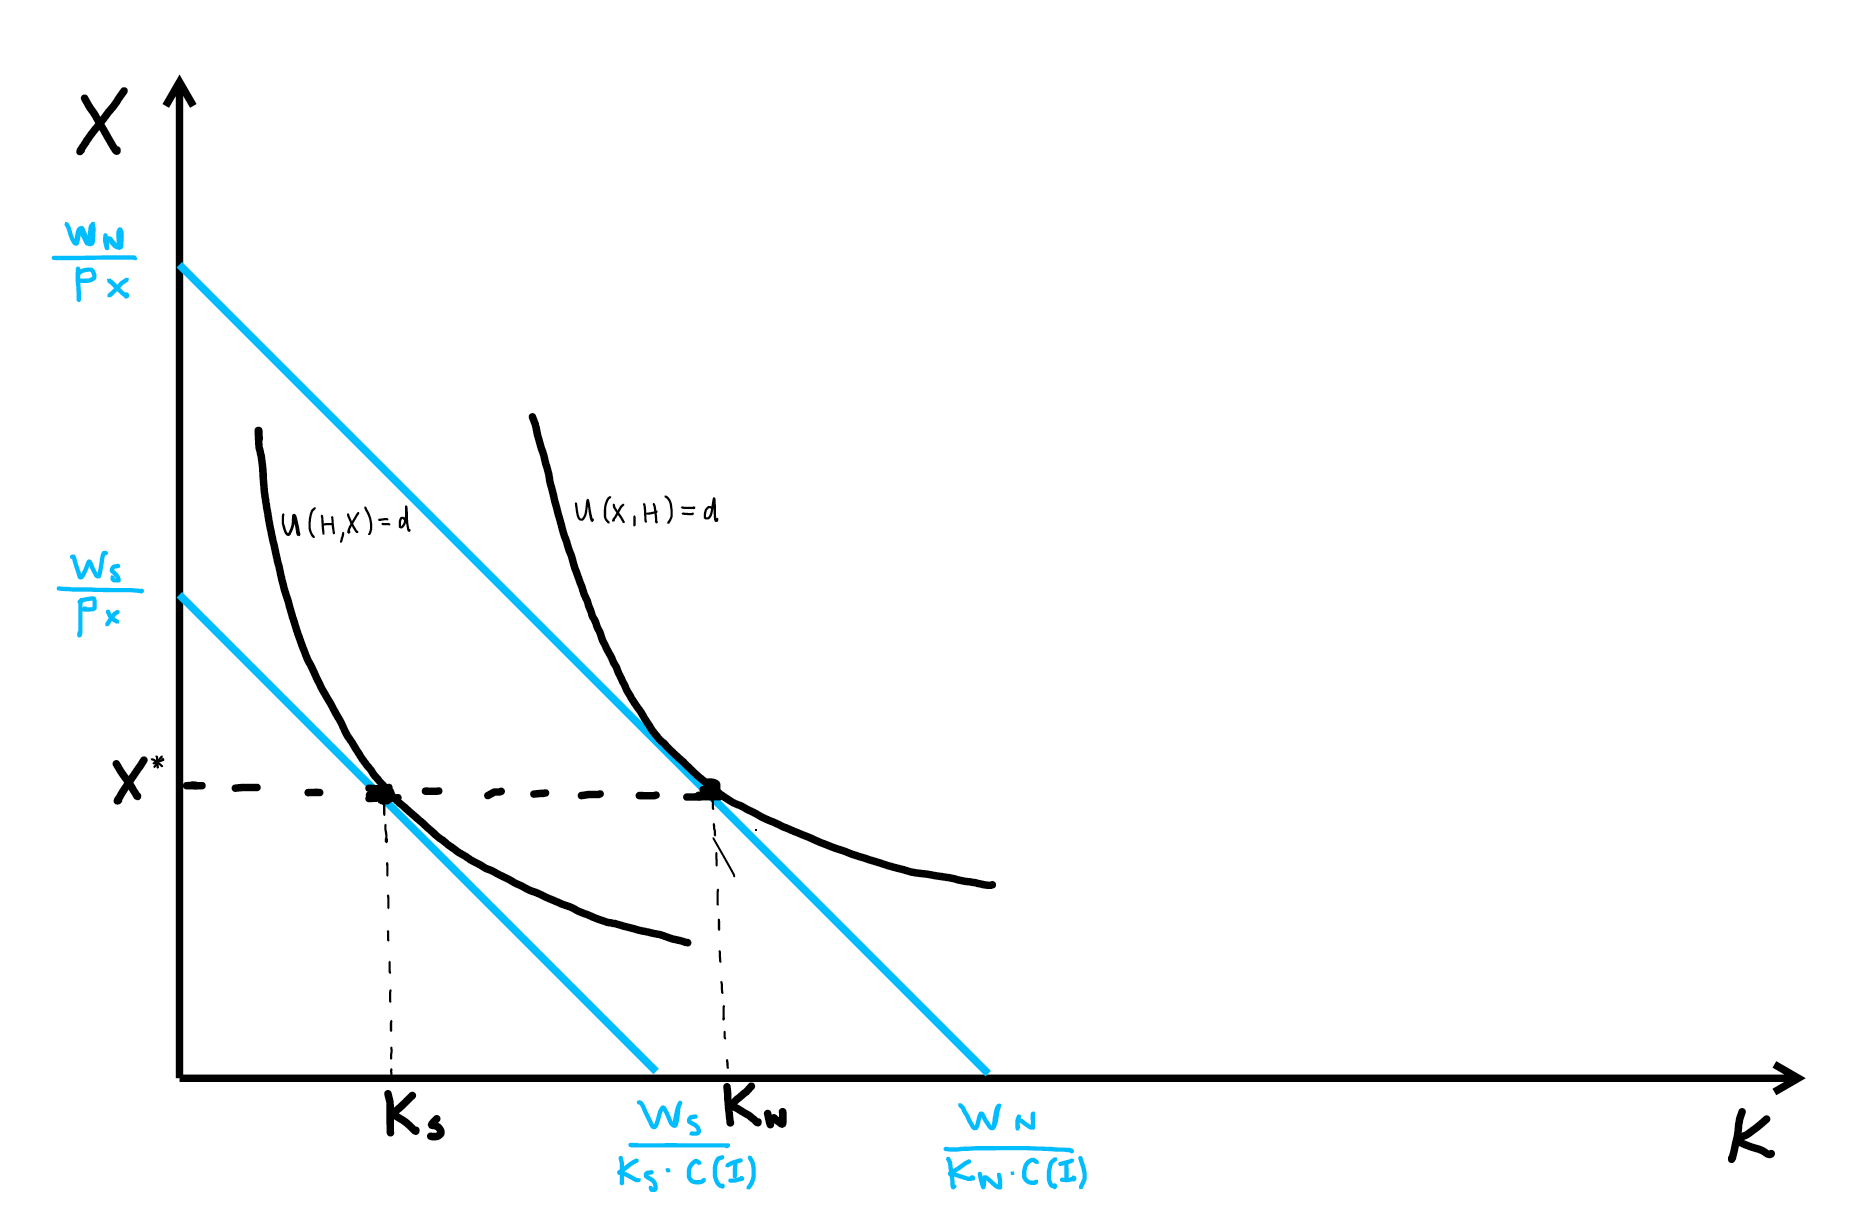
\includegraphics[width=\textwidth]{2-a}
\caption{2-a}
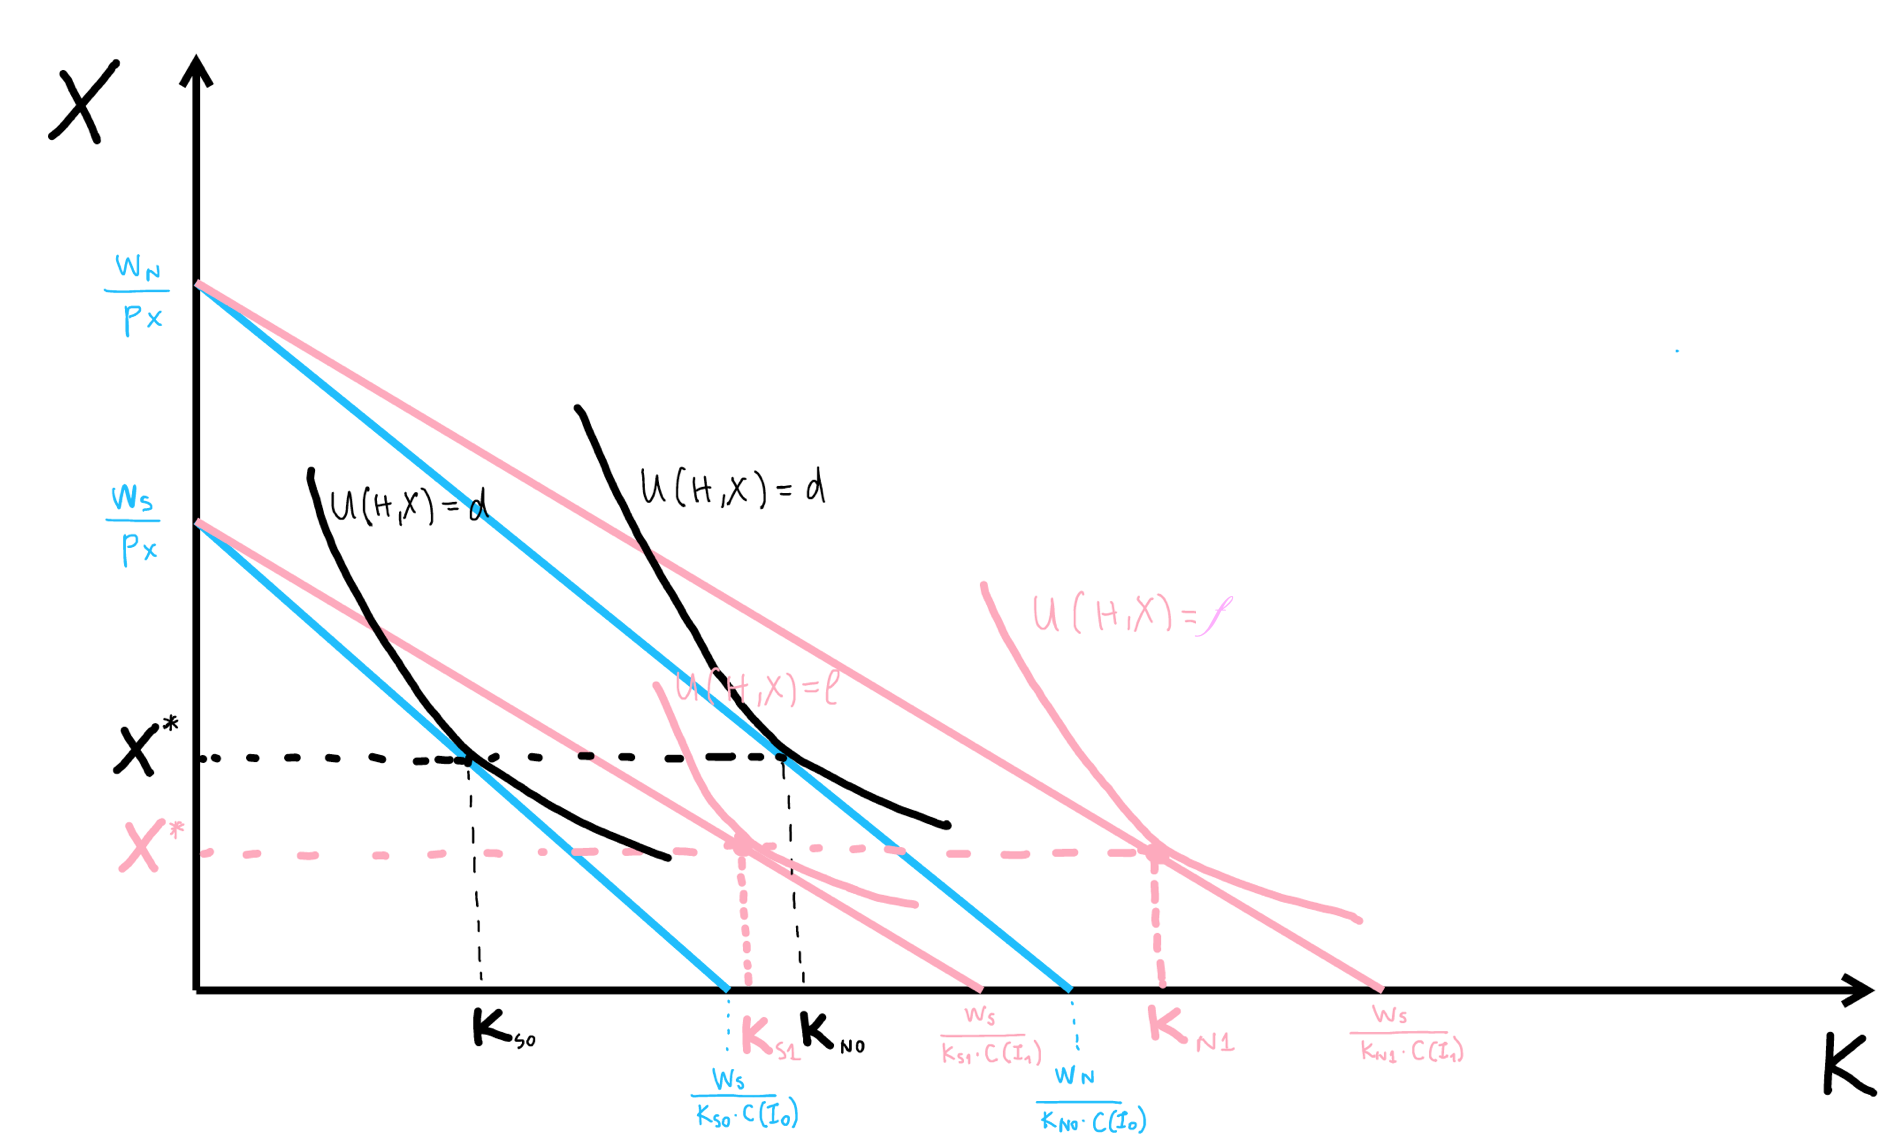
\includegraphics[width=\textwidth]{2-b}
\caption{2-b}
\end{figure}

\begin{figure}
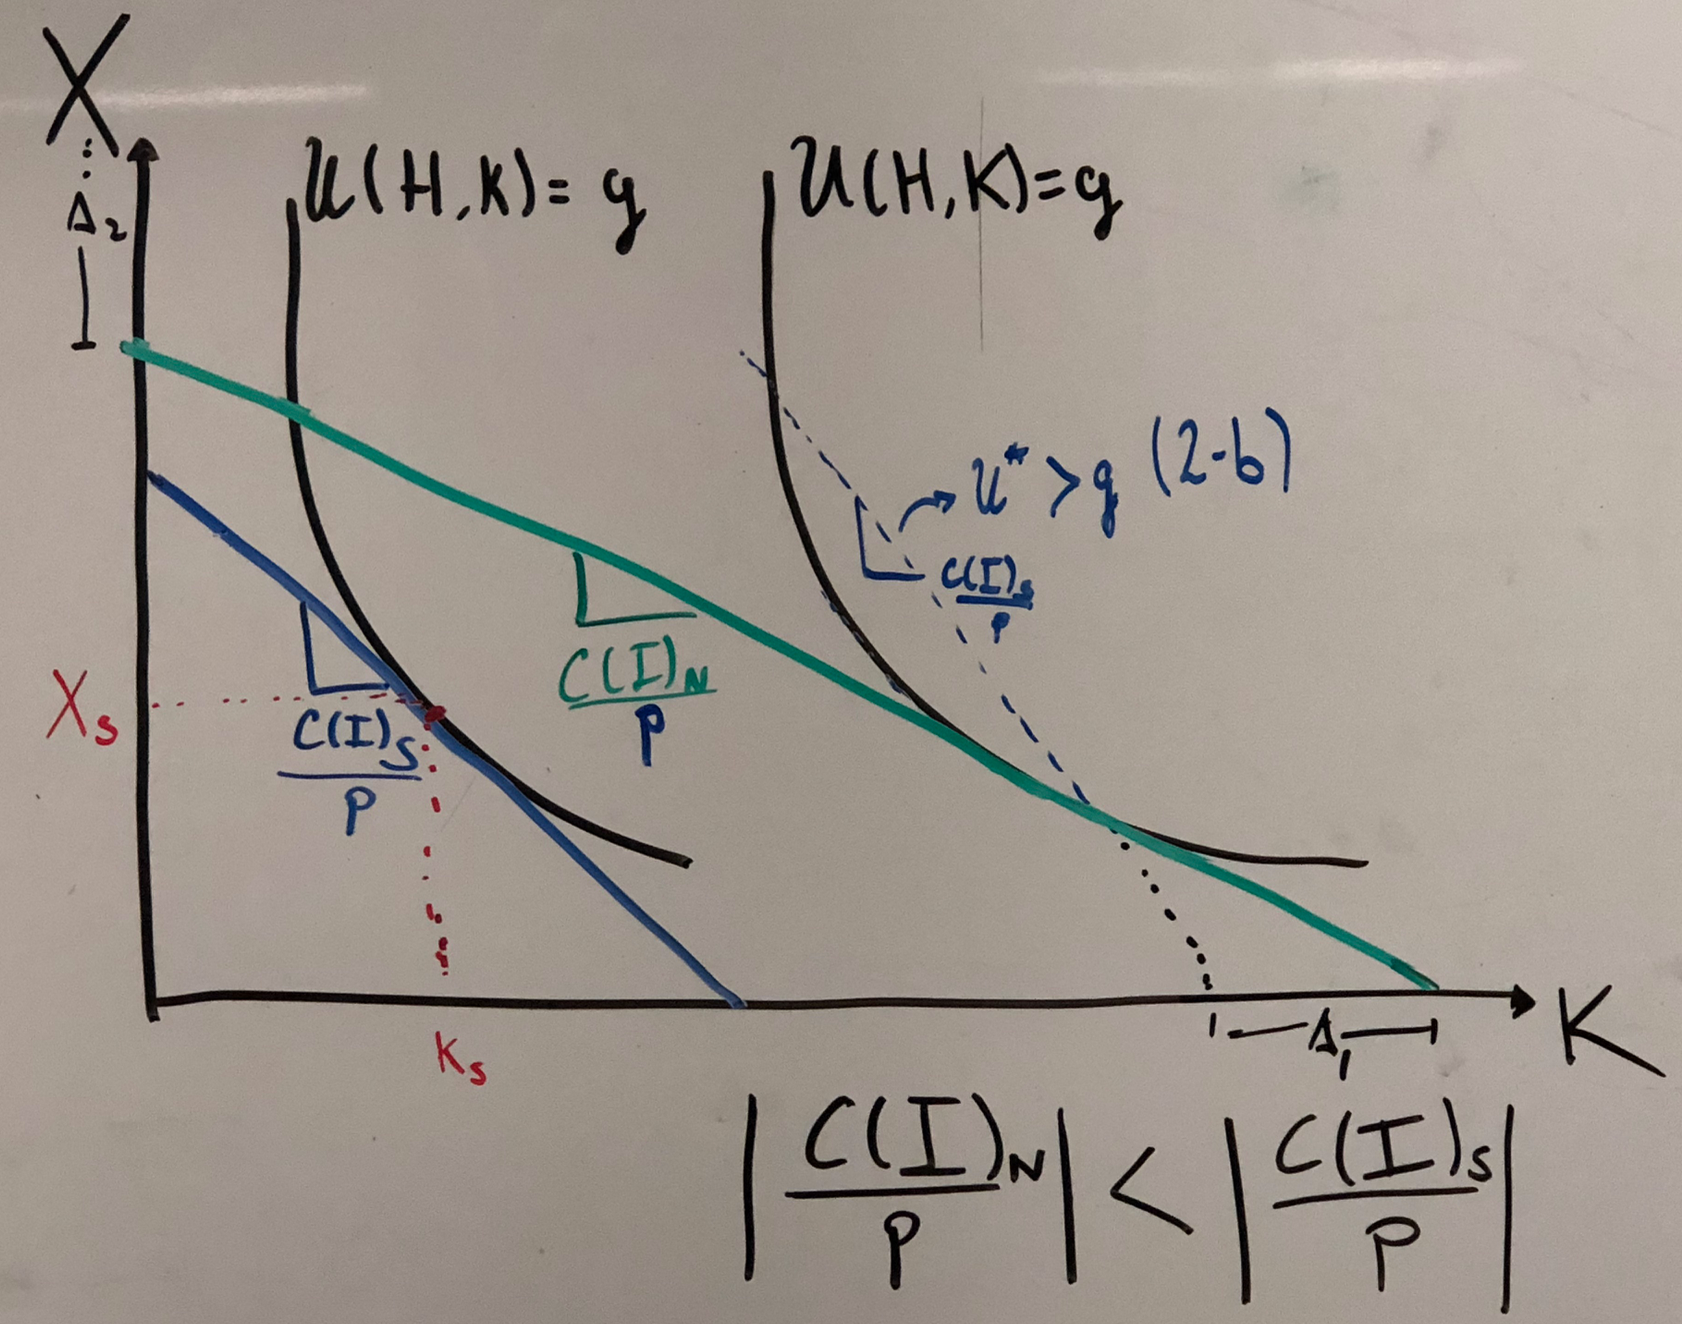
\includegraphics[width=\textwidth]{2-c}
\caption{2-c}

\end{figure}

\begin{align*}
\end{align*}





\end{document}